% Chapter 1

\chapter{State-of-the-Art} % Write in your own chapter title
\label{SoA}
%\addtotoc{State of the Arts}
\lhead{\emph{State of the Art}} % Write in your own chapter title to set the page header

\section{Photonics interconnect}
\subsection{Transmitter}
\subsubsection{Lasers}
\subsubsection{Microring Resonators}
\subsubsection{Modulators}
\subsection{Receiver}
\subsubsection{Optical waveguides}
\subsubsection{Photodetectors}
A naive, intrusive and costly method to measure the power consumption of each device is to connect it to a  power meter. Apparently, this approach is practically unfeasible because of high cost and too much technical intervention on the power supply. Therefore, Kim et al.~\cite{Kim09Ubicomp} propose a so-called ViridiScope system to replace part of the power meters by indirect sensors to detect the environmental parameters around the monitored devices and deduce their power state. In this monitoring system, devices with stable loads can be monitored by indirect sensors such as light intensity sensors, acoustic sensors, etc., while devices with variable loads are attached to a magnetometer  or a direct power meter. A power meter is also installed at the main power line to measure the aggregate power consumption and an algorithm is developed to disaggregate this power to the corresponding devices.
An overview on the power estimation based on sensors and meters is presented in the following. 

\textbf{Magnetometer}: The magnetic field around device $i$ is sampled at 100~Hz and the signal $s_i(t)$ is formed from the standard deviation over one second sliding window. The corresponding power consumption correlated to this signal is estimated as:
\begin{equation}\label{eqA1}
x_i(t) = \alpha_i s_i(t)+\beta_i,
\end{equation}
where $\alpha_i$, $\beta_i$ are the calibration parameters. The magnetic field analysis method is also applied in \cite{Rowe2010}, but combined with electric field, as illustrated in Figure~\ref{fig:A1}. The electric field is generated from the difference of voltages, i.e. a strong electric field may be generated even when the device does not draw current, while magnetic field variations correspond to the changes in power consumption. Therefore, the electric field can be used to determine if the device is powered or not.

\begin{figure}
\centering
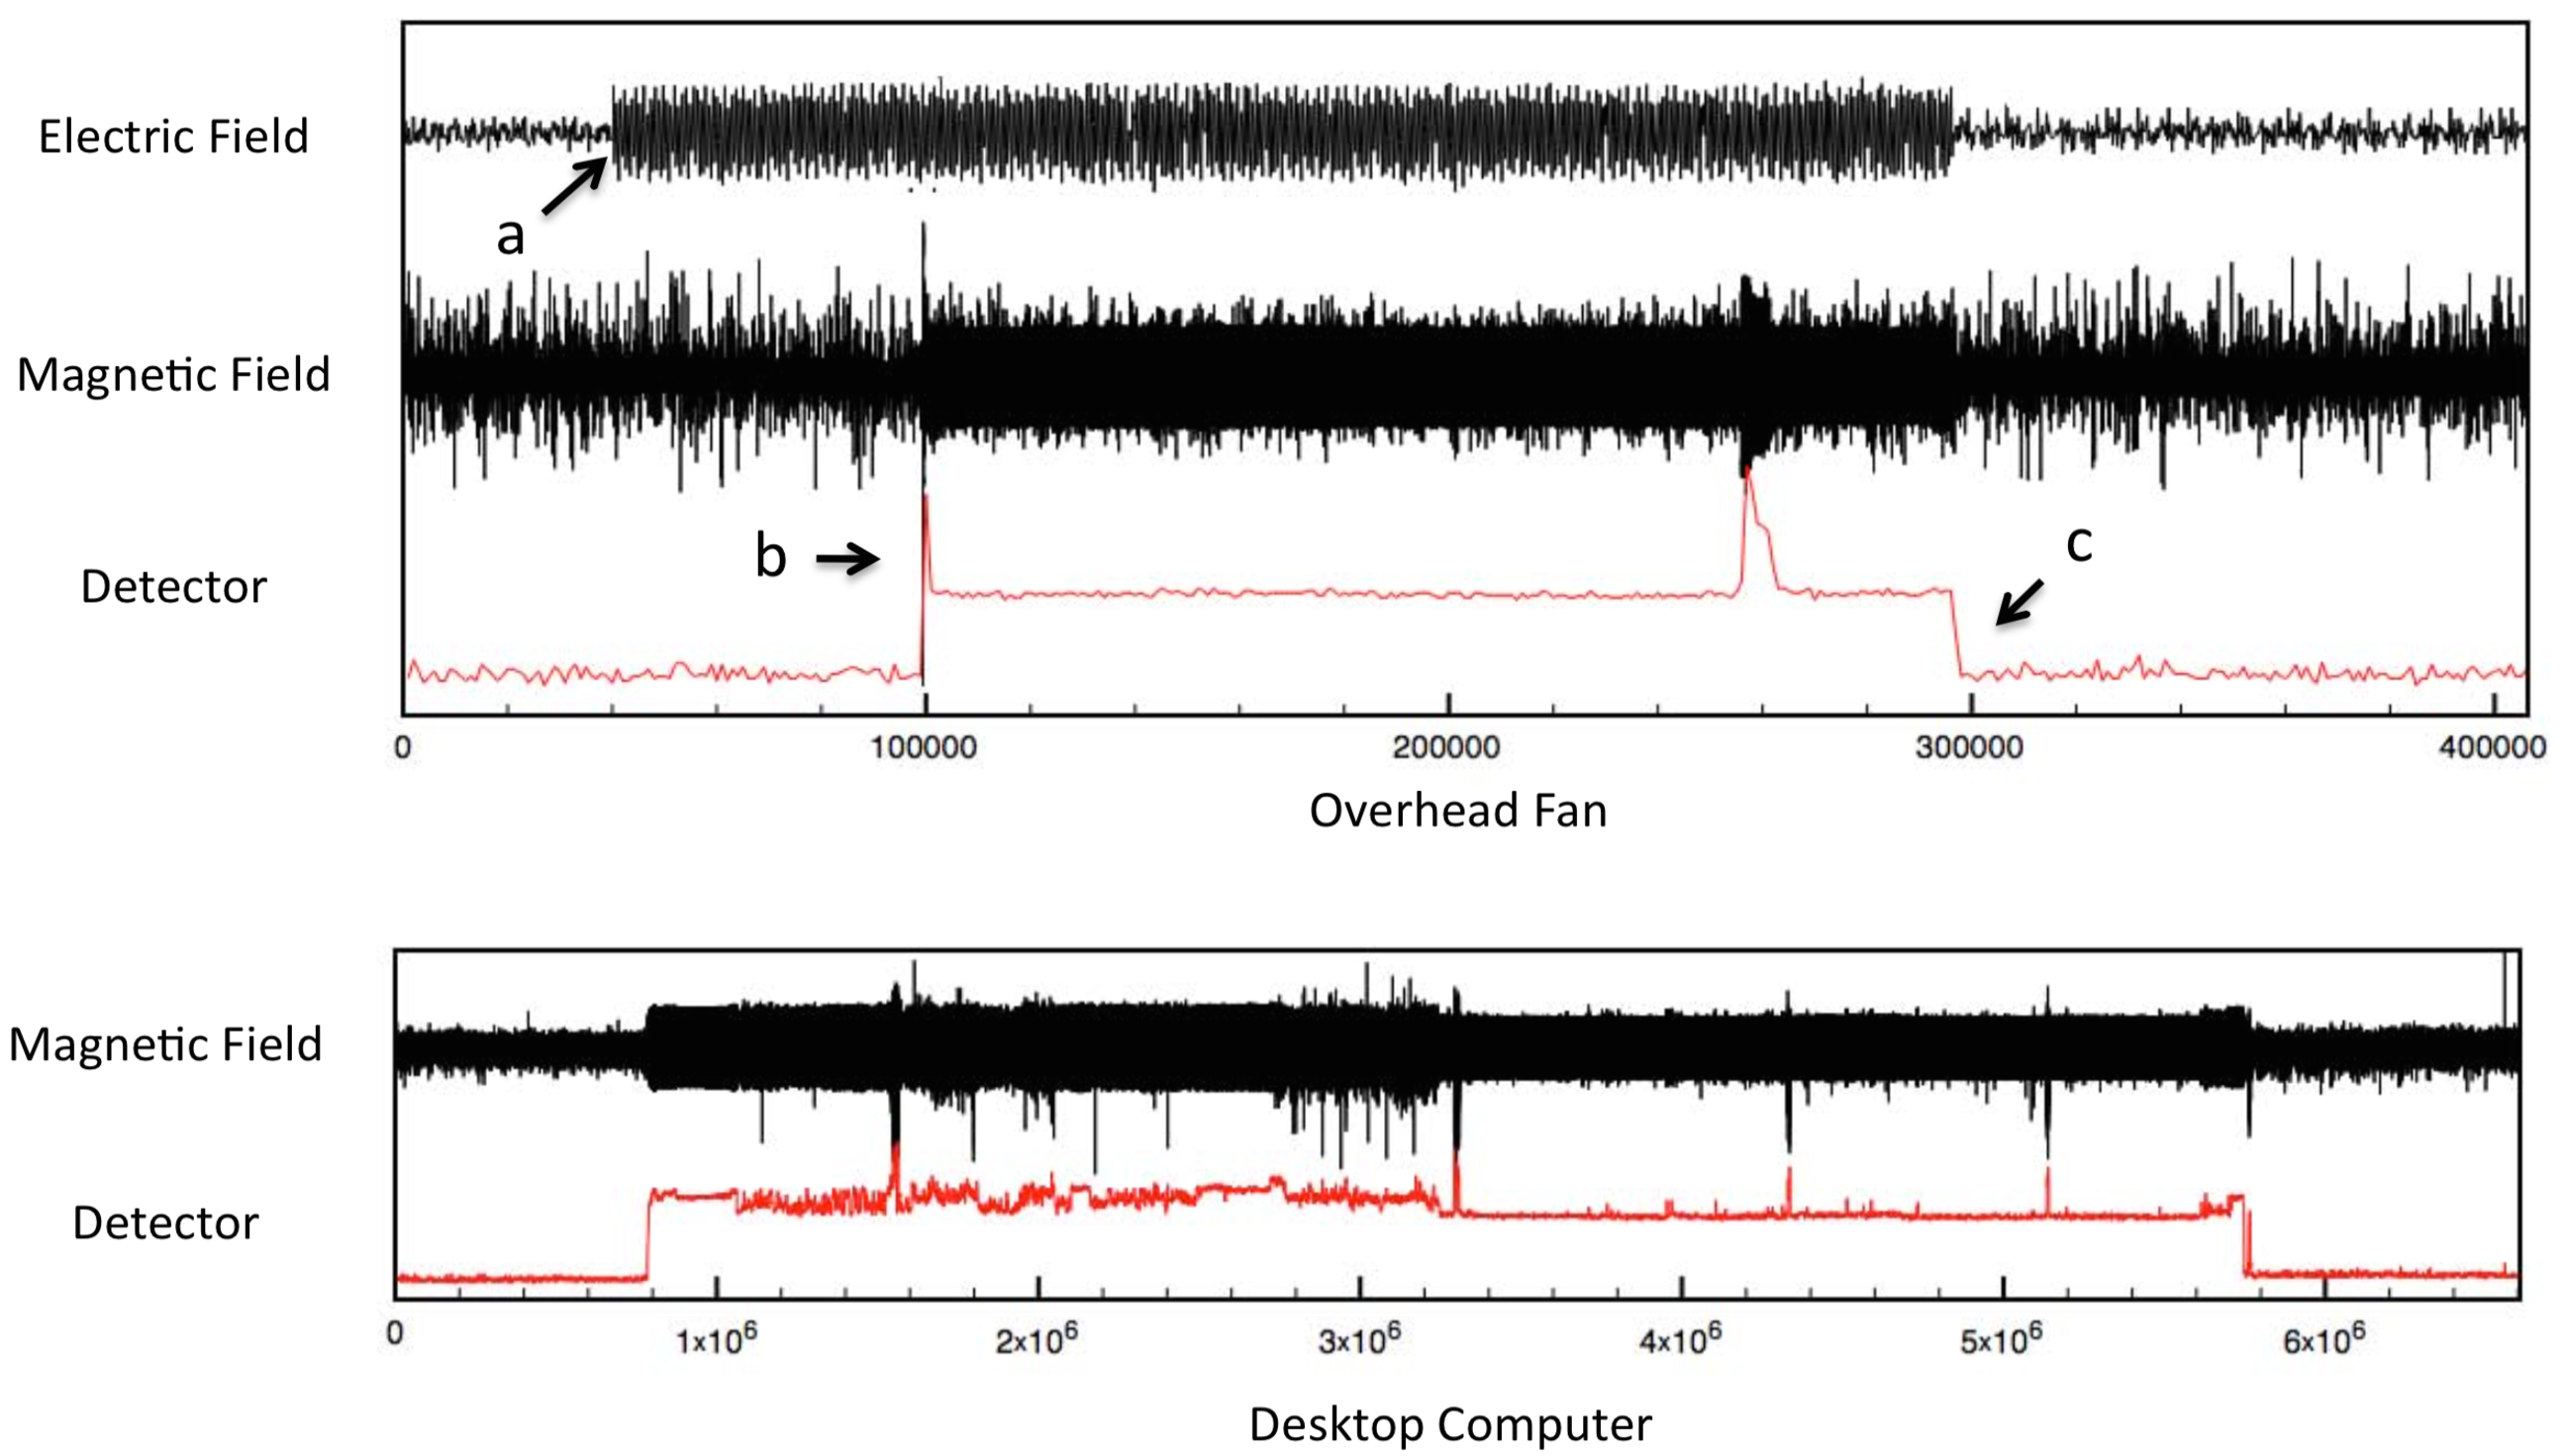
\includegraphics[width=0.8\textwidth]{./chapters/chapter2/images/EMFdetector.pdf} 
\caption{Electromagnetic field waveform. Top: Overhead fan is powered up at point (a), switched on at point (b) and switched off at point (c). Bottom: Variations in magnetic field near by a desktop computer~\cite{Rowe2010}.} 
\label{fig:A1} 
\end{figure}
%---------------------------------

\textbf{Environment monitoring sensors}: To estimate the power consumption of the devices with a limit number of power states, environment monitoring sensors, such as light or acoustic sensors, can be deployed. Denote $s_{ij}(t)$ a boolean indicator of the internal state $j$ of device $i$, the power consumption is estimated by:
\begin{equation}\label{eqA2}
x_i(t) = \sum_{j=1}^{M_i}{w_{ij}.s_{ij}(t)},
\end{equation}
where $M_i$ is the number of internal states of  device $i$ and $w_{ij}$  the average power demand of state $j$.

\textbf{Direct power meter}: There are still other devices monitored by a direct power meter and their power consumption is directly read from the meter. For device $i$,
\begin{equation}\label{eqA3}
x_i(t)=\tilde{x}_i(t),
\end{equation}
where $\tilde{x}_i(t)$ is the signal from the meter connected to device $i$.

\textbf{Uninstrumented devices}: Because of a large number of electrical loads in homes and buildings, some of them cannot be monitored by any meter or sensor. They are called uninstrumented devices. Their total power consumption can be considered as consumed by a unique device. Denote $w_i$ as the total power demand of these devices, their power consumption is estimated from the operating state as
\begin{equation}\label{eqA4}
x_i(t)=w_i s_i(t),
\end{equation}
where $s_i(t)$ indicates if the uninstrumented devices are present in the configuration or not.

Obviously, the total power consumption in home or building is the sum of the power consumption of all devices plus some noise and is defined as
\begin{equation}\label{eqAA5}
\begin{split}
 &x(t)=\sum_{i=1}^{N}{x_i(t)}+n(t)\\
\mbox{where}& \\
 &x_i(t)=\begin{cases}
\alpha_is_i(t)+\beta_i \mbox{: magnetometers}\\
\sum_{j=1}^{M_i}{w_{ij}s_{ij}(t)} \mbox{: light/acoustic sensors}\\
w_is_i(t) \mbox{: uninstrumented}\\
\tilde{x}_i(t) \mbox{: direct meter input}
\end{cases}
\end{split}
\end{equation}
where $N$ is the number of devices and $n(t)$ is a noise. To estimate the power demand of each device, i.e. $w_{ij}$ if monitored by sensors and $w_i$ if uninstrumented, as well as the calibration parameters $\alpha_i,\beta_i$, the following numerical optimization problem formulated from equations \eqref{eqA1}, \eqref{eqA2}, \eqref{eqA3}, \eqref{eqA4} needs to be solved:
\begin{equation}\label{eqA5}
 \min_\theta{\parallel x(t)-\sum_{i=1}^{N}{x_i(t)}\parallel},
\end{equation}
where $\theta$ is a vector containing all variables of power demand and calibration parameters, $\parallel . \parallel$ denotes the $l1$-norm or least absolute value regression solving for the median value. An example of power disaggregation in ViridiScope is represented in Figure~\ref{fig:A2}.

\begin{figure}
\centering
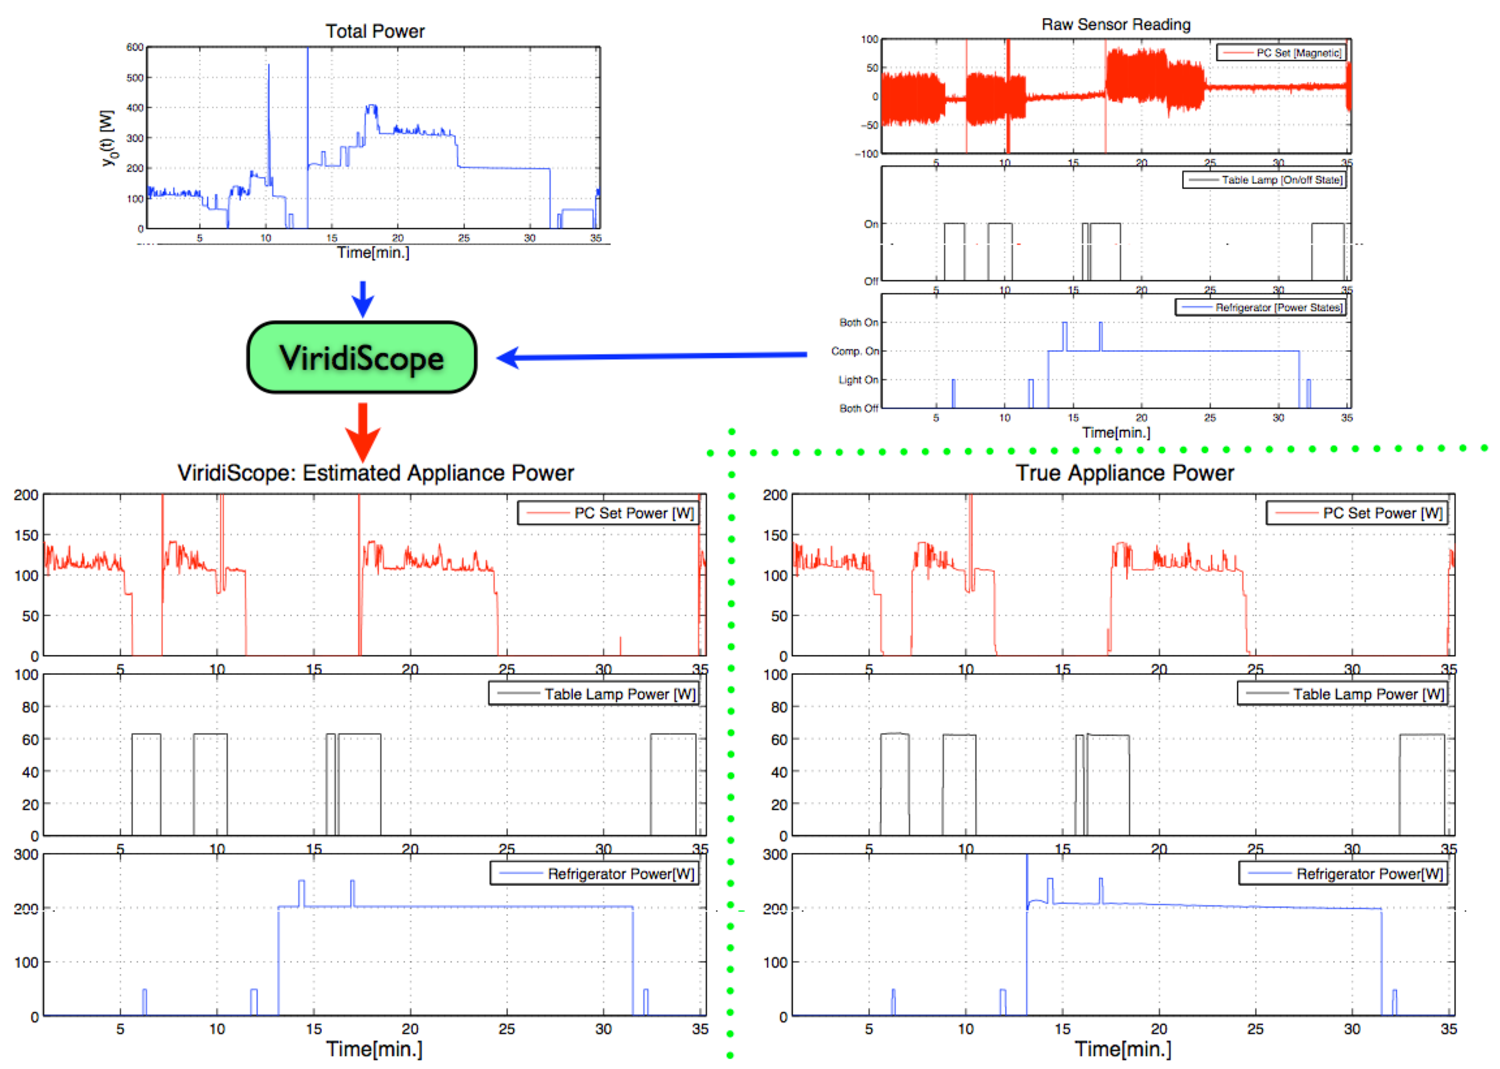
\includegraphics[width=1\textwidth]{./chapters/chapter2/images/ViridiScope_extract.pdf} 
\caption{The ViridiScope system considers the total power consumption, magnetic field signal and internal power state information to estimate the power consumption of each device by solving an $l1$-norm minimization problem~\cite{Kim09Ubicomp}.} 
\label{fig:A2} 
\end{figure}
%---------------------------------

Despite showing a high accuracy ($>90\%$) in the experiment \cite{Kim09Ubicomp}, ViridiScope still has some drawbacks. The first one is that the uninstrumented devices are assumed to consume a constant power, while this power can vary depending on the type of devices. The second limitation relates to the large amount of sensors necessary for deployment to reduce the number of uninstrumented devices and increase the accuracy of the system. 

Similar to ViridiScope, in~\cite{Jung2010,Jung2014}, the authors propose to use binary sensors to detect the on/off state of the energy consumers inside the buildings and then disaggregate the total power consumption to each one. The fundamental difference between this method and ViridiScope is to use the binary sensors providing the on/off state instead of raw data. All devices are assumed to consume a stable power level during their operation. That is the reason why the power consumption of the variable loads or multi-state devices cannot be accurately estimated. To increase the accuracy, the length of observation window used to estimate the power consumption of each device needs to be short enough. Besides, if the on/off sequences of more than two devices are synchronized, the power cannot be disaggregated. In this case, to reach a desired accuracy, some additional power meters are placed to the necessary electrical circuit branches, as illustrated in Figure~\ref{fig:A3}. In this example, because the on/off sequences of devices $x_2$ and $x_5$ are synchronized, their power is impossible to estimate if they are connected to the same power meter as in the left topology and topology 2. In contrast, in topology 1, these devices are connected to different circuit power meters, the disaggregation process can give a better performance. 

\begin{figure}
\centering
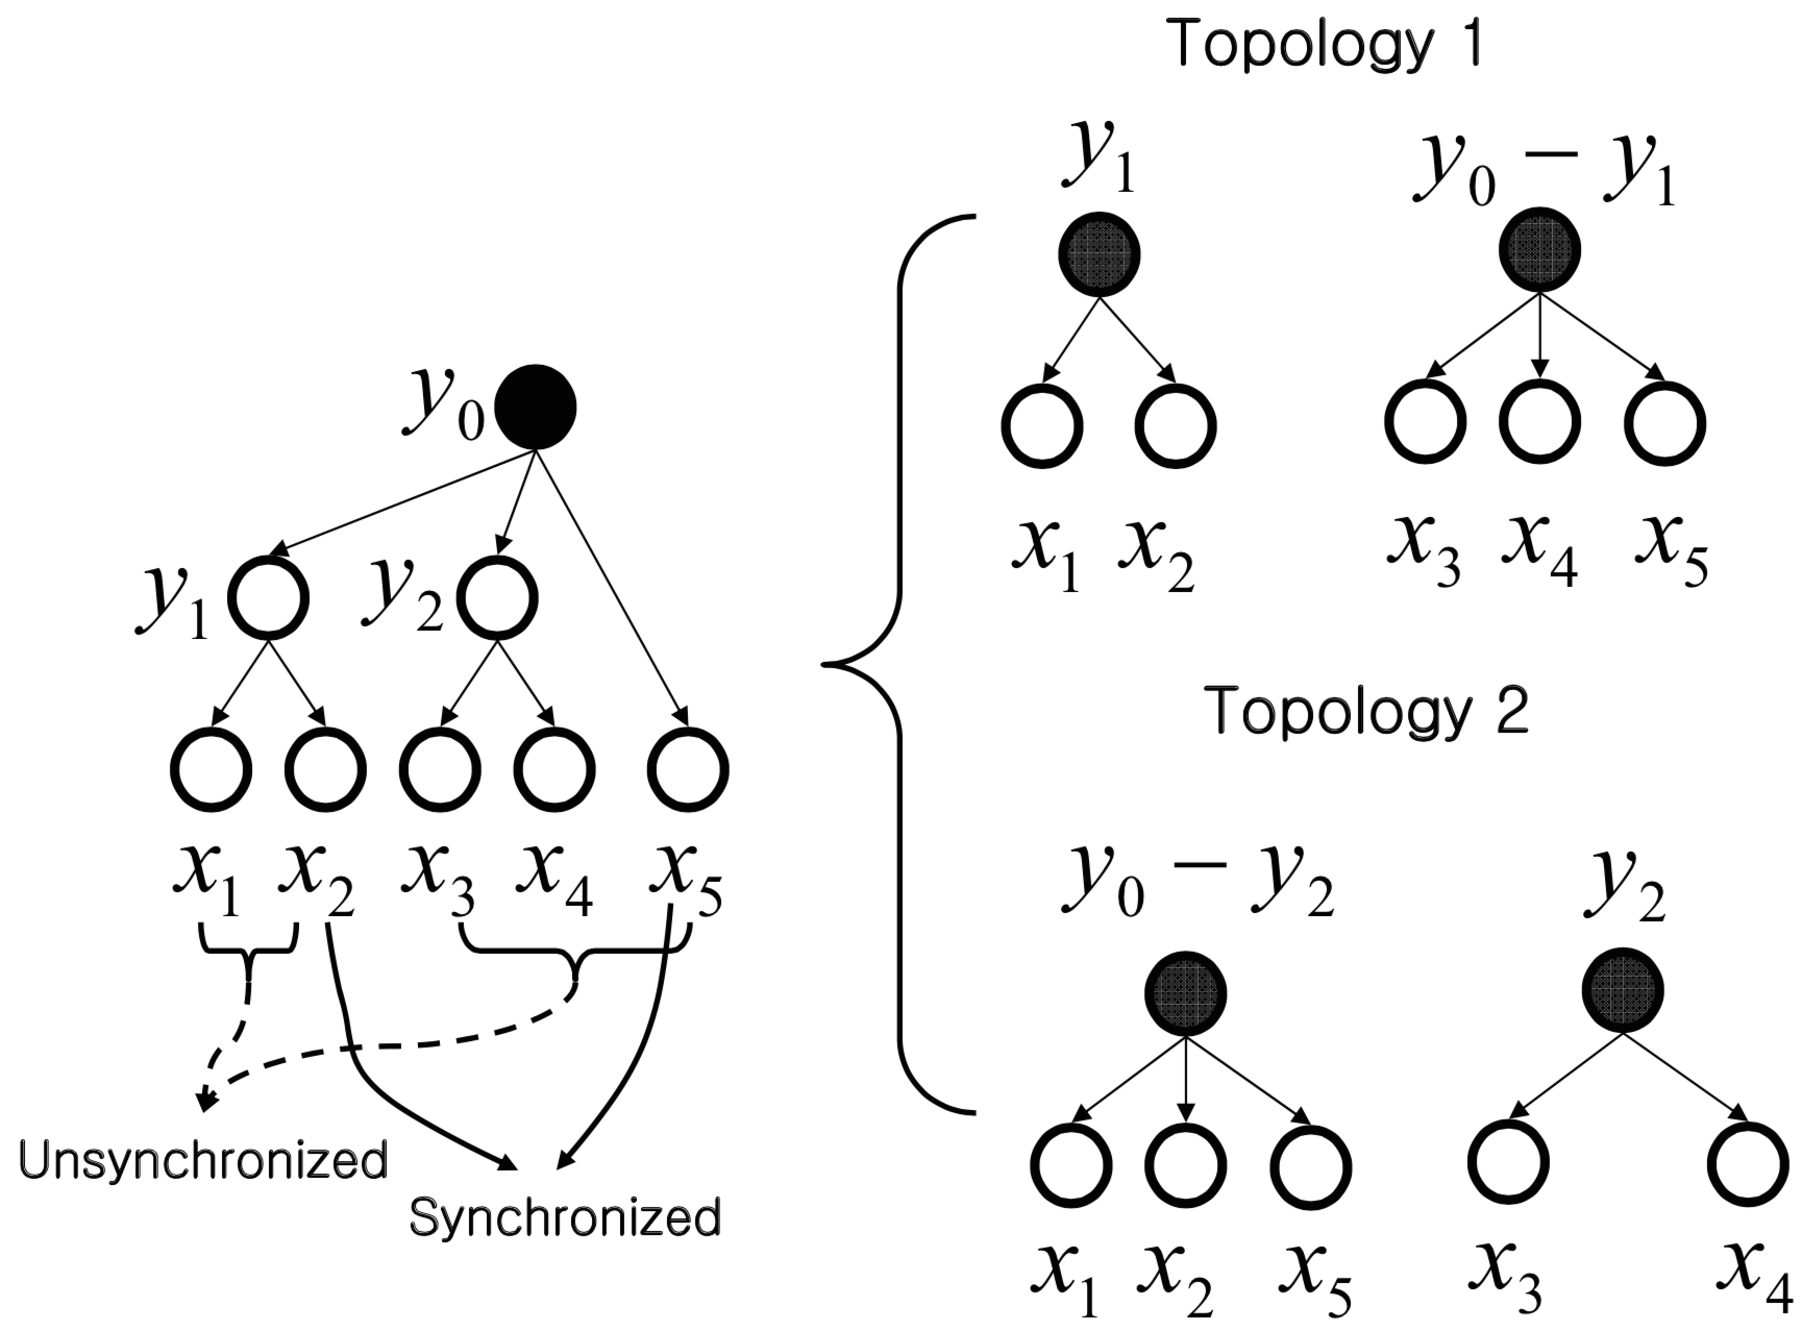
\includegraphics[width=.6\textwidth]{./chapters/chapter2/images/submeters.pdf} 
\caption{Power meter topology. The left topology uses only one power meter (dark node) at the main power supply while topology 1 and 2 use two additional power meters at the electrical circuit branches~\cite{Jung2010}.} 
\label{fig:A3} 
\end{figure}
%---------------------------------

A shortcoming of the research in \cite{Jung2010,Jung2014} is to ignore the presence of the \textit{ghost power} coming from the uninstrumented devices, that has strong effect on the performance when Beckel et al.~\cite{Beckel2012} apply this method to the Reference Energy Disaggregation Dataset (REDD)~\cite{Kolter11redd}. To overcome this problem, they assume to add  an always-on \textit{virtual ghost power consumer} to the set of monitored devices. They also assume that all devices are perfectly monitored by the binary sensors. By this way, the disaggregation can play a better performance, defined by the difference between the estimated power and real power consumption of each device.



